\subsection{Logical View}

\begin{figure}[h!]
\begin{center}
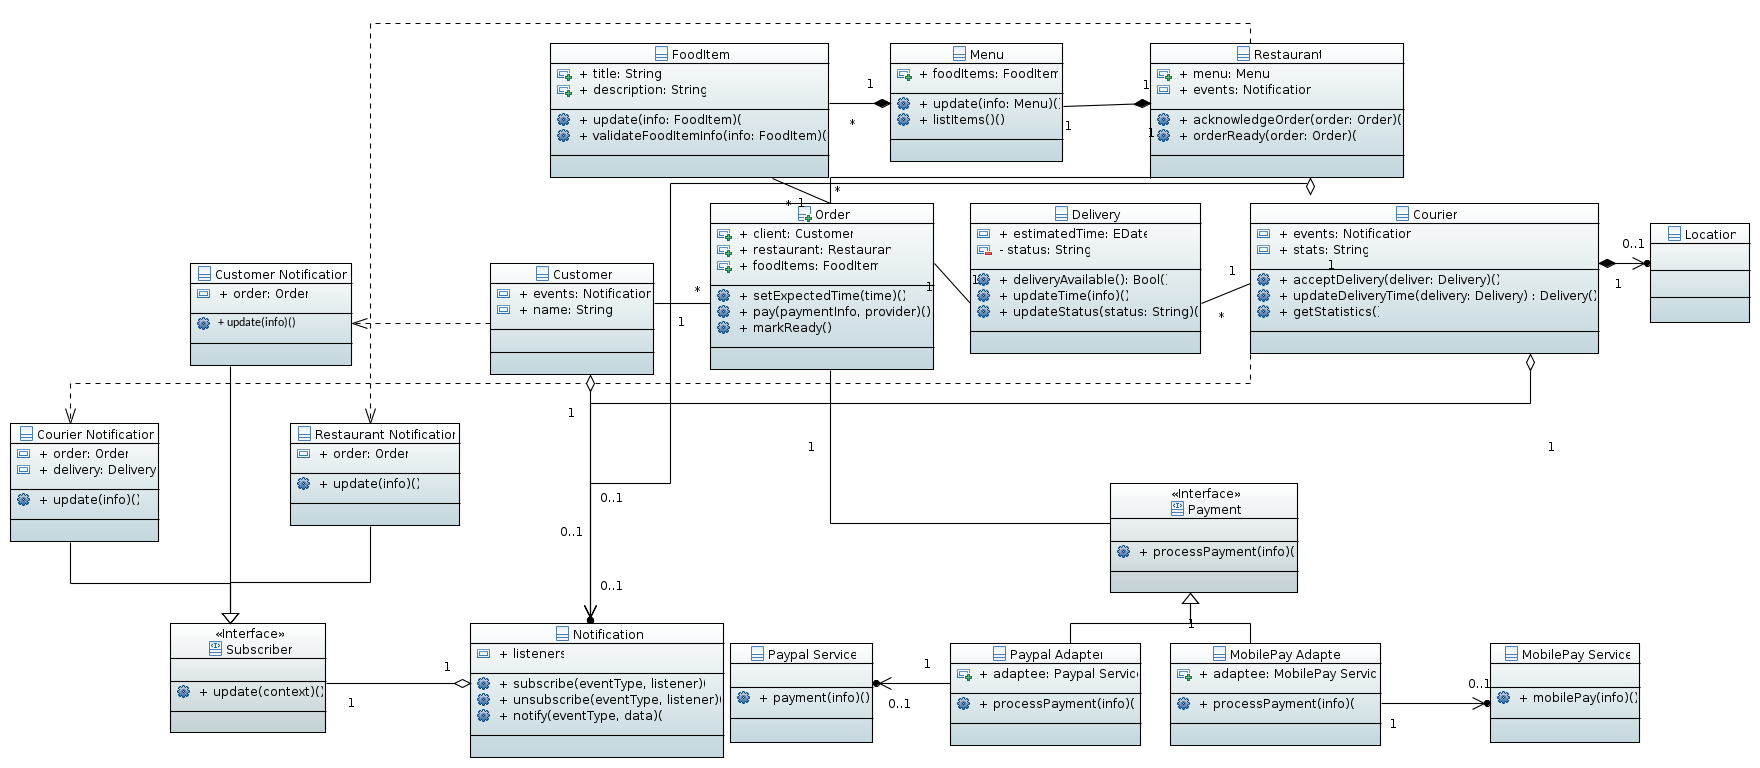
\includegraphics[scale=0.25]{FIGS/ClassDiagram.PNG}
    \caption{Class Diagram}
    \label{fi7g:class_diag}
\end{center}
\end{figure}

The class diagram presented represents the most abstract level of the architecture. All clients, Restaurant, Customer and Courier implement an MVC architectural style which is not depicted in the class diagram to not overload it. This is a higher level diagram, in section \label{seq_diag} all classes needed will be used.

\subsubsection{Classes definition}
\textbf{Courier} represents the system's courier entity, it holds some statistics and its current location and is able to accept and update deliveries. \textbf{Location} is just a position in space that cannot exist by itself. \textbf{Order} is an order created by a customer in the system, binding the customer to a list of items from a restaurant through a payment operation. \textbf{Delivery} is an order ready to be delivered to the customer by a courier, once a restaurant confirms it is ready. \textbf{Payment} is an abstract class adapting the specific payment method. \textbf{Restaurant} represents a restaurant's functionality in the system, it holds a menu and can acknowledge orders from customers and set orders as ready to be delivered. \textbf{Menu} is a collection of food items bound to a restaurant that can be updated and show all the elements in it. \textbf{FoodItem} is each food item defined by a restaurant which can be ordered by a customer, it has some title and description information and can be updated. \textbf{Customer} represents a client in the system, it can place new orders and has some personal information associated with it. \textbf{Notification} represents an event in the system that is originated in one of the main entities (Customer, Restaurant or Courier) and sent to another, notifying of some change in the system.

\subsubsection{Classes Associations}
\textbf{Courier} associates with \textbf{Location} through a composition since a \textit{courier owns its current location and the location has no meaning outside the context of the courier} (e.g. not shared with any other entity). When a courier object is deleted, the location associated with it is deleted too.  
This rule explained above applies to the \textbf{Restaurant}-\textbf{Menu} composition association and to the \textbf{Restaurant}-\textbf{FoodItem}.

The rest are normal associations, each with their different multiplicities.

\subsubsection{Design patterns}

A few design patterns have been considered for the architecture presented in this document.
For the \textbf{Payment} process, since it is stated that an external service will be used, an \textit{Adapter} pattern is used because the \textit{third-party services are already implemented}. Hence, the \textibf{Payment} class is no other than an interface which is implemented by the two services mentioned in the system specification. Each carries out the specific payment process required by each end service.

The notification system has been thought of as an event-based communication, implemented with the \textit{Observer} pattern. This enables the system \textit{to differentiate where to receive notifications from, allowing only the specific classes to receive notifications from those that should push notifications to them.} 